%%%%%%%%%%%%%%%%%%%%%%%%%%%%%%%%%%%%%%%%%
% Diaz Essay
% LaTeX Template
% Version 2.0 (13/1/19)
%
% This template originates from:
% http://www.LaTeXTemplates.com
%
% Authors:
% Vel (vel@LaTeXTemplates.com)
% Nicolas Diaz (nsdiaz@uc.cl)
%
% License:
% CC BY-NC-SA 3.0 (http://creativecommons.org/licenses/by-nc-sa/3.0/)
%
%%%%%%%%%%%%%%%%%%%%%%%%%%%%%%%%%%%%%%%%%

%----------------------------------------------------------------------------------------
%	PACKAGES AND OTHER DOCUMENT CONFIGURATIONS
%----------------------------------------------------------------------------------------


\documentclass[11pt]{diazessay} % Font size (can be 10pt, 11pt or 12pt)
\usepackage{listings}
\usepackage[utf8]{inputenc}
\usepackage{listingsutf8}



\usepackage{color}
\definecolor{gray}{rgb}{0.4,0.4,0.4}
\definecolor{darkblue}{rgb}{0.0,0.0,0.6}
\definecolor{cyan}{rgb}{0.0,0.6,0.6}

\lstset{
	basicstyle=\ttfamily,
	columns=fullflexible,
	showstringspaces=false,
	commentstyle=\color{gray}\upshape
}

\lstdefinelanguage{XML}
{
	morestring=[b]",
	morestring=[s]{>}{<},
	morecomment=[s]{<?}{?>},
	stringstyle=\color{black},
	identifierstyle=\color{darkblue},
	keywordstyle=\color{cyan},
	morekeywords={xmlns,version,type}% list your attributes here
}

%----------------------------------------------------------------------------------------
%	TITLE SECTION
%----------------------------------------------------------------------------------------

\title{\textbf{Ejemplos de casos en el Big Data \\ Informe preliminar}} % Title and subtitle

\author{\textbf{Bases de Datos Avanzadas} \\ \textit{Escuela Superior Informática (UCLM)}} % Author and institution

\date{\today} % Date, use \date{} for no date

%----------------------------------------------------------------------------------------

\begin{document}

\maketitle % Print the title section


%----------------------------------------------------------------------------------------
%	ABSTRACT AND KEYWORDS
%----------------------------------------------------------------------------------------

%\renewcommand{\abstractname}{Summary} % Uncomment to change the name of the abstract to something else

\begin{abstract}
	
	%%%%% RESUMEN  %%%%%
En este informe, se hablará sobre que es el \textbf{\textit{Big Data}}, sus principales características y ventajas, los tipos de datos que maneja el uso de esta tecnología. Al igual de como se lleva acabo la gestión de la información (\textit{datos}).\\

Y finalmente, se describirán una serie de proyectos que gracias a la utilización de esta tecnología han tenido \textbf{éxito}, y otros que han acabado en \textbf{fracaso}.
\end{abstract}

\hspace*{3.6mm}\textit{Keywords:} \textit{Big Data}, \textit{Éxito}, \textit{Fracaso}, \textit{Calidad de los datos}

\vspace{20pt} % Vertical whitespace between the abstract and first section

%----------------------------------------------------------------------------------------
%	ESSAY BODY
%----------------------------------------------------------------------------------------
\newpage
\section*{Introducción}

El \textbf{Big Data} \cite{wiki-data} (\textit{macro datos, datos masivos, inteligencia de datos}), se conoce como el análisis masivo de datos. Esto es una cantidad de datos tan sumamente grande, que las aplicaciones que se dedicaban al  procesamiento de datos que tradicionalmente se venían usando no son capaces de tratar y poner en valor en un tiempo razonable. Este  término ha estado en uso desde la década de \textit{1990}.\\
Este término también hace referencia, a las nuevas tecnologías que hacen posible el almacenamiento y procesamiento de datos, además del uso que se hace de la información obtenida a través de ellas.\\

\subsection*{Tipos de datos que existen}
A continuación, se dará una breve explicación de los tipos de datos existentes \cite{wiki-ucm}, y de los cuales hace uso esta tecnología (\textbf{\textit{Big Data}}).

\subsubsection*{Datos estructurados}
Este tipo de datos se suelen usar en el tratamiento de datos. Ya que sus principales características son que pueden ser almacenados en tablas, y que tienen definido su formato.\\
Algunos datos de este tipo son:

\begin{itemize}
	\item \textbf{Números.}
	\item \textbf{Cadenas de caracteres.}
	\item \textbf{Fechas.}
\end{itemize}

\subsubsection*{Datos semiestructurados}
Los \textbf{\textit{datos semiestructurados}} tienen una tipo de estructura, pero esta no es lo suficientemente regular, como para permitir su gestión y estructuración como si fuese similar a los datos estructurados.
Este tipo de datos, posee ciertos patrones comunes que lo describen y dan información sobre las relaciones entre los mismos.\\
Un ejemplo de utilización, sería el lenguaje de marcas \textit{HTML}, el cual sirve para el desarrollo de paginas web, donde estas pautas son representadas por su sistema de etiquetas.

\subsubsection*{Datos no estructurados}
Este tipo de datos, se trata  de datos que han sido obtenidos en su formato original. Estos no se encuentran especificados en ningún formato, el cual permita que sean almacenados como se almacenarían los anteriores tipos de datos (\textit{estructurados} y \textit{semiestructurados}). Ya que no disponen de una estructura definida (longitud, formato, etc) para poder desglosar la información.\\
Estos datos se pueden encontrar, por ejemplo: en presentaciones (\textit{PowerPoints}), correos, documentos de texto \textit{(Word, PDF, documentos de google}, etc).



\newpage
\section*{Características principales}
Las características principales del \textit{\textbf{Big Data}} en este caso son \textbf{siete}, también son conocidas como las \textit{"V" del Big Data}. Este nombre se debe a que las siete características comienzan por la letra "V".\\ 
Estas son las siguientes:

\begin{enumerate}
	\item \textbf{Valor}: A la hora de extraer una gran cantidad de datos, frecuentemente se extrae algo de valor entre ellos. La pregunta que se hacen en este ambito, es como extraer con mas frecuencia y de manera eficiente, el valor de los datos. Ya que el valor es sin duda una cualidad fundamental en su análisis.
	
	\item \textbf{Velocidad}: La velocidad es algo fundamental en este ámbito, ya que es necesario que la información sea captada al instante. Ya que por ejemplo, si se quiere captar una serie de noticias, y en cambio estas no llegan hasta un tiempo sobrepasado. Esto puede hacer que pierden valor e interés. Por ello cada vez los algoritmos que se encargan de captar la información cada vez son mas rápidos y trabajan en tiempo real, a la vez esto hace que estos tipos de algoritmos sean más complejos.
	
	\item \textbf{Variabilidad}: En este ámbito (de los \textit{macro datos}), la información varía de forma constante. Es por ello que también varían bastante los mecanismos de tratamientos de datos, ya que estos no pueden ser fijos, y necesitan un control periódico.
	
	\item \textbf{Variedad}: ya que los datos son captados desde diversas fuentes y también se encuentran en distintos formatos. Además la proporción de datos no estructurados en cuanto a los estructurados (\textit{tradicionales}), cada vez es mayor. Por tanto, esto provoca la necesidad de utilizar nuevas tecnologías de tratamiento de datos.
	
	\item \textbf{Visualización}:Por ejemplo, convertir cientos de archivos de información en un único gráfico, que muestre de forma clara una serie de conclusiones o resúmenes, de los tipos de datos e información captada.
	
	\item \textbf{Volumen}: Dado que la cantidad de datos generados esta evolucionando de una forma exponencial, esto provoca ue crezcan las bases de datos, y al igual las aplicaciones que se encargan de captar esa información previamente. Como respuesta a estos cambios, se han reducido los costes de almacenamiento.
	
	\item \textbf{Veracidad}: Saber la veracidad de la información que se ha recogido, es algo fundamental para obtener unos datos de \textit{\textbf{calidad}}.  Esta característica puede influir en gran parte en conseguir ventajas competitivas dentro del ámbito del \textit{Big Data}.
\end{enumerate}


\newpage
\section*{Ciclo de gestión de los datos}
El ciclo de gestión de información del \textit{\textbf{Big Data}}, es el siguiente:

\begin{enumerate}
	\item \textbf{Captura de información}: Existen varios métodos, como: Web Scraping, esta es una técnica que durante programas que extraen información de sitios Web. Y la gestión de información con diversas APIs.
	
	\item \textbf{Almacenamiento}: Dependiendo de lo que se tenga pensado optar, se puede optar desde archivos de hojas de cálculo hasta sistemas NoSQL. Estos sistemas permiten el almacenamiento de información no estructurada, de una forma rápida y flexible.
	
	\item \textbf{Tratamiento}: Una vez que los datos han sido capturados y almacenados, deben de ser tratados. Este proceso dependerá del tipo de información y de su uso. Se puede extraer patrones de ellos mediante la utilización del \textit{\textbf{machine learning}}, esto es el desarrollo de diversas técnicas que tienen como finalidad que las maquinas basen su comportamiento en base a ejemplos que se les agencian. Todo ello mediante lenguajes de programación como \textit{R} y \textit{Python}.
	
	\item \textbf{Puesta en valor}: Los datos solo garantizan conocimiento cuando han sido analizados y tratados de forma adecuada. Esto hace que el valor no se encuentre en los propios datos, si no en la relación que hay entre estos.\\
	Esta relación es la que permite extraer patrones, los cuales forman el conocimiento en todo tipo de ámbitos. Por ejemplo, el valor pude ser una visualización a partir de un grafico, donde se lleve a cabo un análisis.\\
	Por lo tanto, con esto nos referimos a algo que realmente de sentido a todo el proceso que se ha llevado a cabo hasta llegar aquí.
\end{enumerate}

\begin{figure}[h!]
	\centering
	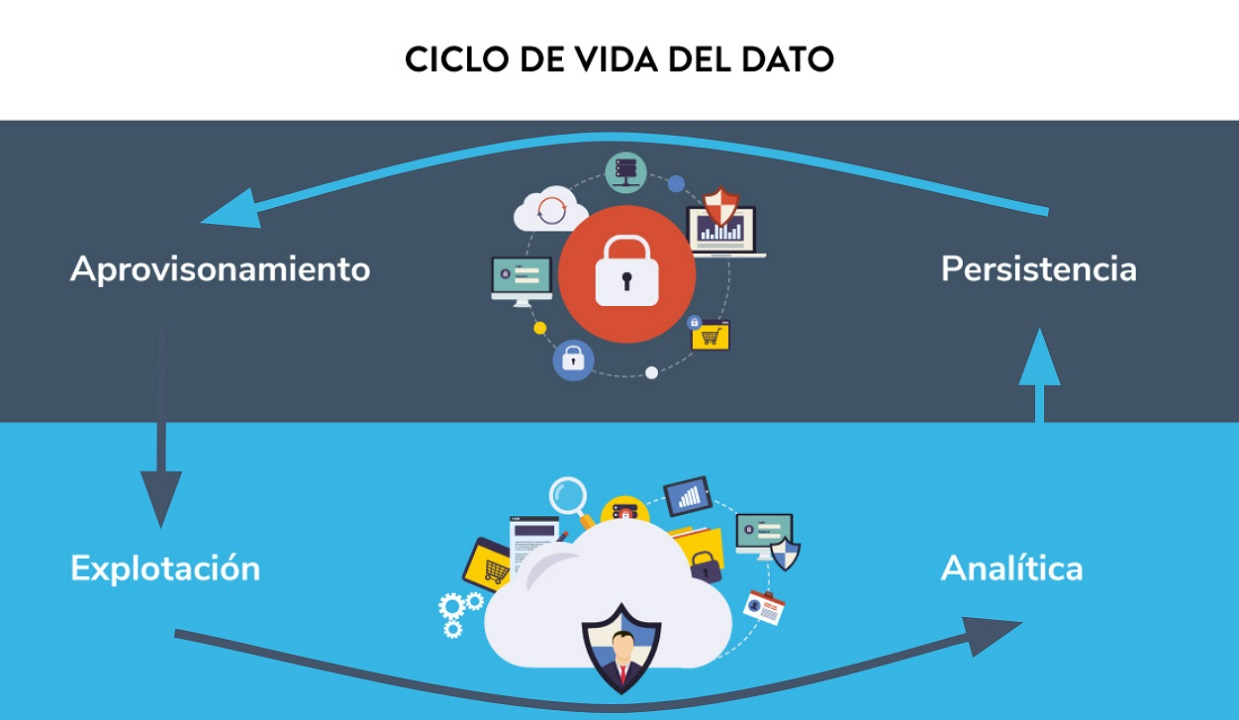
\includegraphics[width=\linewidth]{ciclo.jpg}
	\caption{Representación ciclo de vida del \textit{dato}.}
	\label{fig:ciclo-dato}
\end{figure}


\newpage
\section*{Ejemplos de casos en el Big Data}
A continuación, se nombrarán algunos casos de éxito y de fracaso dentro del ámbito del \textit{\textbf{Big Data}}.\\

\subsection*{Casos de éxito:}

\subsubsection*{Amazon}
\textit{Amazon} \cite{wiki-amazon} es una de las principales compañias de comercio electrónico, basa buena parte de su éxito en conocer de antemano lo que necesitan sus clientes.

\begin{figure}[h!]
	\centering
	
\includegraphics[width=50mm]{amazon.png}
	\caption{Logotipo de \textit{Amazon}.}
	\label{fig:amazon}
\end{figure}

Si entras en la página de esta empresa, se puede observar como, sugiere artículos que van a ser de gran interés para el cliente. Este proceso se lleva a cabo mediante el uso de inteligencia de datos. Esta analiza los factores de individuales de cada usuario como sus hábitos de compra, intereses y otros más generales como tendencias del momento o pautas de conducta. Juntan todo esta información y ofrecen una serie de productos sugeridos o relacionados con compras que el cliente ya ha hecho o que haya pensado hacer en otro momento.\\
En la Figura \ref{fig:proceso} se puede ver representado este proceso.\\


\subsubsection*{Spotify}
\textit{Spotify} \cite{wiki-spotify} en una de las principales aplicaciones multiplataforma de escuchar música en streaming. Utiliza los datos para bajar los datos individualizados de sus usuarios más llamativos para lanzar con ellos una campaña global masiva. Su plan consistió en buscar la complicidad del gran público. Y lo consiguieron mostrando curiosidades o rarezas del comportamiento de algunos de sus usuarios. Los cuales habían detectado a través de los \textit{macrodatos}.\\

\begin{figure}[h!]
	\centering
	
\includegraphics[width=50mm]{spotify.png}
	\caption{Logotipo de \textit{Spotify}.}
	\label{fig:spotify}
\end{figure}

\clearpage
Como por ejemplo: mostrar en grandes carteles publicitarios, anuncios como:\\
\textit{«Querida persona que reprodujo “El perdón” 42 veces en el Día de San Valentín, ¿qué hiciste?»}\\
\textit{«Queridas 3.749 personas que reprodujeron “It’s the end of the world as we know it” el día del Brexit, estamos con vosotros»}\\

Todo esto provocó que gran parte de los usuarios, se descargasen y utilizasen esta aplicación. y le dio a esta empresa colocarse en la cima de su ámbito o tipo de aplicaciones similares.\\
En la Figura \ref{fig:proceso} se puede ver representado este proceso.\\


\subsubsection*{Netflix}
\textit{Netflix} \cite{wiki-netflix} es una de las principales empresas de entretenimiento a nivel mundial. cuyo servicio principal es la distribución de contenidos audiovisuales a través de una plataforma en línea o servicio de VOD (video bajo demanda) por \textit{streaming}.

\begin{figure}[h!]
	\centering
	
\includegraphics[width=50mm]{netflix.png}
	\caption{Logotipo de \textit{Netflix}.}
	\label{fig:netflix}
\end{figure}

Uno de sus mayores factores de éxito, es su magistral uso de los \textit{macro datos} para crear nuevos contenidos para sus usuarios, cuyos hábitos de consumo y preferencias son observados al detalle para descubrir qué es lo que van a querer ver a continuación en base a patrones predictivos.\\

Por ejemplo: Con este proceso han llegado a crear muchas de sus series. En concreto, la serie \textit{House of Cards}: mediante la observación de que a muchos de sus usuarios les gustaban contenidos que incluyeran poder, política, drama y sensualidad entre sus características principales. Y también que les gustaba como actor Kevin Spacey. Así, dieron con la fórmula y mezclaron en la trama de esta serie todos estos ingredientes poniendo como protagonista principal a Kevin Spacey. También aplicaron este proceso a otras series muy famosas de su cartelera, como es el caso de \textit{Stranger Things}.\\
En la Figura \ref{fig:proceso} se puede ver representado como se lleva a cabo este proceso.\\
\clearpage

\begin{figure}[h!]
	\centering
	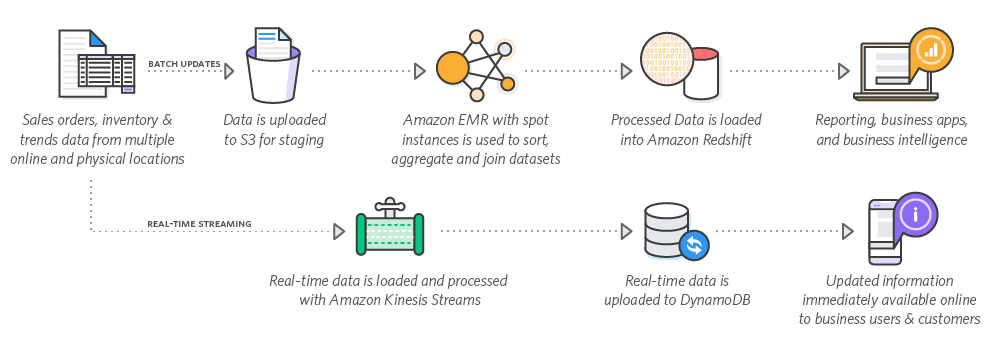
\includegraphics[width=\linewidth]{proceso.png}
	\caption{Representación de adquisición y tratamiento de la información de los usuarios en estos tipos de plataformas.}
	\label{fig:proceso}
\end{figure}


\subsection*{Casos de fracaso}
Según las estadísticas el \textbf{65} \% de los proyectos que utilizan tecnologías de \textit{\textbf{Big Data}} fracasan. Esto se debe principalmente a la gran inversión de \textbf{presupuesto} que un proyecto de este tipo necesita. También a la falta de profesionales especificados en este ámbito. Y por último a la calidad que necesitan los datos. Uno de los ejemplos de fracaso de un proyecto de este tipo, es el siguiente:\\
 










%----------------------------------------------------------------------------------------
%	BIBLIOGRAPHY
%----------------------------------------------------------------------------------------
\clearpage
\bibliographystyle{abbrv}

\bibliography{sample.bib}

%----------------------------------------------------------------------------------------

\end{document}
